% Created by tikzDevice version 0.12.3 on 2020-01-31 13:13:19
% !TEX encoding = UTF-8 Unicode
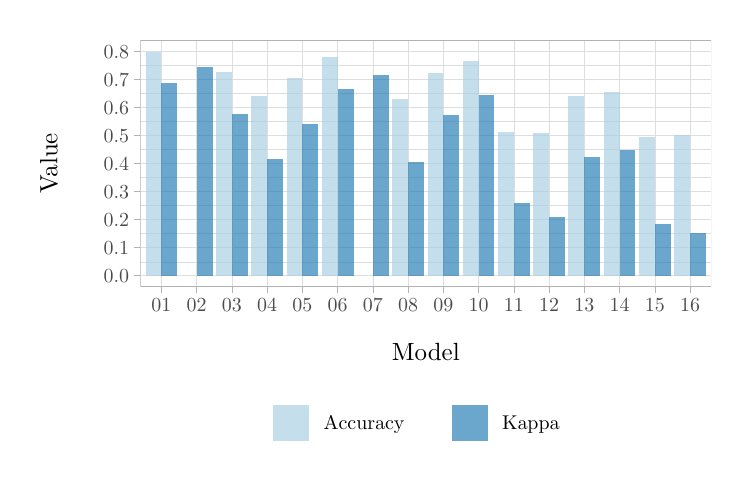
\begin{tikzpicture}[x=1pt,y=1pt]
\definecolor{fillColor}{RGB}{255,255,255}
\path[use as bounding box,fill=fillColor,fill opacity=0.00] (0,0) rectangle (251.50,158.99);
\begin{scope}
\path[clip] (  0.00,  0.00) rectangle (251.50,158.99);
\definecolor{drawColor}{RGB}{255,255,255}
\definecolor{fillColor}{RGB}{255,255,255}

\path[draw=drawColor,line width= 0.5pt,line join=round,line cap=round,fill=fillColor] (  0.00,  0.00) rectangle (251.50,158.99);
\end{scope}
\begin{scope}
\path[clip] ( 40.70, 65.31) rectangle (247.00,154.49);
\definecolor{fillColor}{RGB}{255,255,255}

\path[fill=fillColor] ( 40.70, 65.31) rectangle (247.00,154.49);
\definecolor{drawColor}{gray}{0.87}

\path[draw=drawColor,line width= 0.1pt,line join=round] ( 40.70, 74.43) --
	(247.00, 74.43);

\path[draw=drawColor,line width= 0.1pt,line join=round] ( 40.70, 84.57) --
	(247.00, 84.57);

\path[draw=drawColor,line width= 0.1pt,line join=round] ( 40.70, 94.70) --
	(247.00, 94.70);

\path[draw=drawColor,line width= 0.1pt,line join=round] ( 40.70,104.83) --
	(247.00,104.83);

\path[draw=drawColor,line width= 0.1pt,line join=round] ( 40.70,114.97) --
	(247.00,114.97);

\path[draw=drawColor,line width= 0.1pt,line join=round] ( 40.70,125.10) --
	(247.00,125.10);

\path[draw=drawColor,line width= 0.1pt,line join=round] ( 40.70,135.24) --
	(247.00,135.24);

\path[draw=drawColor,line width= 0.1pt,line join=round] ( 40.70,145.37) --
	(247.00,145.37);

\path[draw=drawColor,line width= 0.2pt,line join=round] ( 40.70, 69.36) --
	(247.00, 69.36);

\path[draw=drawColor,line width= 0.2pt,line join=round] ( 40.70, 79.50) --
	(247.00, 79.50);

\path[draw=drawColor,line width= 0.2pt,line join=round] ( 40.70, 89.63) --
	(247.00, 89.63);

\path[draw=drawColor,line width= 0.2pt,line join=round] ( 40.70, 99.77) --
	(247.00, 99.77);

\path[draw=drawColor,line width= 0.2pt,line join=round] ( 40.70,109.90) --
	(247.00,109.90);

\path[draw=drawColor,line width= 0.2pt,line join=round] ( 40.70,120.04) --
	(247.00,120.04);

\path[draw=drawColor,line width= 0.2pt,line join=round] ( 40.70,130.17) --
	(247.00,130.17);

\path[draw=drawColor,line width= 0.2pt,line join=round] ( 40.70,140.31) --
	(247.00,140.31);

\path[draw=drawColor,line width= 0.2pt,line join=round] ( 40.70,150.44) --
	(247.00,150.44);

\path[draw=drawColor,line width= 0.2pt,line join=round] ( 48.34, 65.31) --
	( 48.34,154.49);

\path[draw=drawColor,line width= 0.2pt,line join=round] ( 61.07, 65.31) --
	( 61.07,154.49);

\path[draw=drawColor,line width= 0.2pt,line join=round] ( 73.81, 65.31) --
	( 73.81,154.49);

\path[draw=drawColor,line width= 0.2pt,line join=round] ( 86.54, 65.31) --
	( 86.54,154.49);

\path[draw=drawColor,line width= 0.2pt,line join=round] ( 99.28, 65.31) --
	( 99.28,154.49);

\path[draw=drawColor,line width= 0.2pt,line join=round] (112.01, 65.31) --
	(112.01,154.49);

\path[draw=drawColor,line width= 0.2pt,line join=round] (124.75, 65.31) --
	(124.75,154.49);

\path[draw=drawColor,line width= 0.2pt,line join=round] (137.48, 65.31) --
	(137.48,154.49);

\path[draw=drawColor,line width= 0.2pt,line join=round] (150.22, 65.31) --
	(150.22,154.49);

\path[draw=drawColor,line width= 0.2pt,line join=round] (162.95, 65.31) --
	(162.95,154.49);

\path[draw=drawColor,line width= 0.2pt,line join=round] (175.68, 65.31) --
	(175.68,154.49);

\path[draw=drawColor,line width= 0.2pt,line join=round] (188.42, 65.31) --
	(188.42,154.49);

\path[draw=drawColor,line width= 0.2pt,line join=round] (201.15, 65.31) --
	(201.15,154.49);

\path[draw=drawColor,line width= 0.2pt,line join=round] (213.89, 65.31) --
	(213.89,154.49);

\path[draw=drawColor,line width= 0.2pt,line join=round] (226.62, 65.31) --
	(226.62,154.49);

\path[draw=drawColor,line width= 0.2pt,line join=round] (239.36, 65.31) --
	(239.36,154.49);
\definecolor{fillColor}{RGB}{31,120,180}

\path[fill=fillColor,fill opacity=0.66] ( 48.34, 69.36) rectangle ( 54.07,139.03);
\definecolor{fillColor}{RGB}{166,206,227}

\path[fill=fillColor,fill opacity=0.66] ( 42.61, 69.36) rectangle ( 48.34,150.28);
\definecolor{fillColor}{RGB}{31,120,180}

\path[fill=fillColor,fill opacity=0.66] ( 61.07, 69.36) rectangle ( 66.80,144.87);

\path[fill=fillColor,fill opacity=0.66] ( 73.81, 69.36) rectangle ( 79.54,127.71);
\definecolor{fillColor}{RGB}{166,206,227}

\path[fill=fillColor,fill opacity=0.66] ( 68.08, 69.36) rectangle ( 73.81,142.96);
\definecolor{fillColor}{RGB}{31,120,180}

\path[fill=fillColor,fill opacity=0.66] ( 86.54, 69.36) rectangle ( 92.27,111.52);
\definecolor{fillColor}{RGB}{166,206,227}

\path[fill=fillColor,fill opacity=0.66] ( 80.81, 69.36) rectangle ( 86.54,134.46);
\definecolor{fillColor}{RGB}{31,120,180}

\path[fill=fillColor,fill opacity=0.66] ( 99.28, 69.36) rectangle (105.01,124.26);
\definecolor{fillColor}{RGB}{166,206,227}

\path[fill=fillColor,fill opacity=0.66] ( 93.55, 69.36) rectangle ( 99.28,140.77);
\definecolor{fillColor}{RGB}{31,120,180}

\path[fill=fillColor,fill opacity=0.66] (112.01, 69.36) rectangle (117.74,136.67);
\definecolor{fillColor}{RGB}{166,206,227}

\path[fill=fillColor,fill opacity=0.66] (106.28, 69.36) rectangle (112.01,148.54);
\definecolor{fillColor}{RGB}{31,120,180}

\path[fill=fillColor,fill opacity=0.66] (124.75, 69.36) rectangle (130.48,141.79);

\path[fill=fillColor,fill opacity=0.66] (137.48, 69.36) rectangle (143.21,110.34);
\definecolor{fillColor}{RGB}{166,206,227}

\path[fill=fillColor,fill opacity=0.66] (131.75, 69.36) rectangle (137.48,133.33);
\definecolor{fillColor}{RGB}{31,120,180}

\path[fill=fillColor,fill opacity=0.66] (150.22, 69.36) rectangle (155.95,127.43);
\definecolor{fillColor}{RGB}{166,206,227}

\path[fill=fillColor,fill opacity=0.66] (144.48, 69.36) rectangle (150.22,142.63);
\definecolor{fillColor}{RGB}{31,120,180}

\path[fill=fillColor,fill opacity=0.66] (162.95, 69.36) rectangle (168.68,134.53);
\definecolor{fillColor}{RGB}{166,206,227}

\path[fill=fillColor,fill opacity=0.66] (157.22, 69.36) rectangle (162.95,146.86);
\definecolor{fillColor}{RGB}{31,120,180}

\path[fill=fillColor,fill opacity=0.66] (175.68, 69.36) rectangle (181.42, 95.57);
\definecolor{fillColor}{RGB}{166,206,227}

\path[fill=fillColor,fill opacity=0.66] (169.95, 69.36) rectangle (175.68,121.22);
\definecolor{fillColor}{RGB}{31,120,180}

\path[fill=fillColor,fill opacity=0.66] (188.42, 69.36) rectangle (194.15, 90.57);
\definecolor{fillColor}{RGB}{166,206,227}

\path[fill=fillColor,fill opacity=0.66] (182.69, 69.36) rectangle (188.42,121.09);
\definecolor{fillColor}{RGB}{31,120,180}

\path[fill=fillColor,fill opacity=0.66] (201.15, 69.36) rectangle (206.88,112.27);
\definecolor{fillColor}{RGB}{166,206,227}

\path[fill=fillColor,fill opacity=0.66] (195.42, 69.36) rectangle (201.15,134.23);
\definecolor{fillColor}{RGB}{31,120,180}

\path[fill=fillColor,fill opacity=0.66] (213.89, 69.36) rectangle (219.62,114.87);
\definecolor{fillColor}{RGB}{166,206,227}

\path[fill=fillColor,fill opacity=0.66] (208.16, 69.36) rectangle (213.89,135.70);
\definecolor{fillColor}{RGB}{31,120,180}

\path[fill=fillColor,fill opacity=0.66] (226.62, 69.36) rectangle (232.35, 88.12);
\definecolor{fillColor}{RGB}{166,206,227}

\path[fill=fillColor,fill opacity=0.66] (220.89, 69.36) rectangle (226.62,119.44);
\definecolor{fillColor}{RGB}{31,120,180}

\path[fill=fillColor,fill opacity=0.66] (239.36, 69.36) rectangle (245.09, 84.86);
\definecolor{fillColor}{RGB}{166,206,227}

\path[fill=fillColor,fill opacity=0.66] (233.63, 69.36) rectangle (239.36,120.04);
\definecolor{drawColor}{gray}{0.70}

\path[draw=drawColor,line width= 0.5pt,line join=round,line cap=round] ( 40.70, 65.31) rectangle (247.00,154.49);
\end{scope}
\begin{scope}
\path[clip] (  0.00,  0.00) rectangle (251.50,158.99);
\definecolor{drawColor}{gray}{0.30}

\node[text=drawColor,anchor=base east,inner sep=0pt, outer sep=0pt, scale=  0.72] at ( 36.65, 66.88) {0.0};

\node[text=drawColor,anchor=base east,inner sep=0pt, outer sep=0pt, scale=  0.72] at ( 36.65, 77.02) {0.1};

\node[text=drawColor,anchor=base east,inner sep=0pt, outer sep=0pt, scale=  0.72] at ( 36.65, 87.15) {0.2};

\node[text=drawColor,anchor=base east,inner sep=0pt, outer sep=0pt, scale=  0.72] at ( 36.65, 97.29) {0.3};

\node[text=drawColor,anchor=base east,inner sep=0pt, outer sep=0pt, scale=  0.72] at ( 36.65,107.42) {0.4};

\node[text=drawColor,anchor=base east,inner sep=0pt, outer sep=0pt, scale=  0.72] at ( 36.65,117.56) {0.5};

\node[text=drawColor,anchor=base east,inner sep=0pt, outer sep=0pt, scale=  0.72] at ( 36.65,127.69) {0.6};

\node[text=drawColor,anchor=base east,inner sep=0pt, outer sep=0pt, scale=  0.72] at ( 36.65,137.83) {0.7};

\node[text=drawColor,anchor=base east,inner sep=0pt, outer sep=0pt, scale=  0.72] at ( 36.65,147.96) {0.8};
\end{scope}
\begin{scope}
\path[clip] (  0.00,  0.00) rectangle (251.50,158.99);
\definecolor{drawColor}{gray}{0.70}

\path[draw=drawColor,line width= 0.2pt,line join=round] ( 38.45, 69.36) --
	( 40.70, 69.36);

\path[draw=drawColor,line width= 0.2pt,line join=round] ( 38.45, 79.50) --
	( 40.70, 79.50);

\path[draw=drawColor,line width= 0.2pt,line join=round] ( 38.45, 89.63) --
	( 40.70, 89.63);

\path[draw=drawColor,line width= 0.2pt,line join=round] ( 38.45, 99.77) --
	( 40.70, 99.77);

\path[draw=drawColor,line width= 0.2pt,line join=round] ( 38.45,109.90) --
	( 40.70,109.90);

\path[draw=drawColor,line width= 0.2pt,line join=round] ( 38.45,120.04) --
	( 40.70,120.04);

\path[draw=drawColor,line width= 0.2pt,line join=round] ( 38.45,130.17) --
	( 40.70,130.17);

\path[draw=drawColor,line width= 0.2pt,line join=round] ( 38.45,140.31) --
	( 40.70,140.31);

\path[draw=drawColor,line width= 0.2pt,line join=round] ( 38.45,150.44) --
	( 40.70,150.44);
\end{scope}
\begin{scope}
\path[clip] (  0.00,  0.00) rectangle (251.50,158.99);
\definecolor{drawColor}{gray}{0.70}

\path[draw=drawColor,line width= 0.2pt,line join=round] ( 48.34, 63.06) --
	( 48.34, 65.31);

\path[draw=drawColor,line width= 0.2pt,line join=round] ( 61.07, 63.06) --
	( 61.07, 65.31);

\path[draw=drawColor,line width= 0.2pt,line join=round] ( 73.81, 63.06) --
	( 73.81, 65.31);

\path[draw=drawColor,line width= 0.2pt,line join=round] ( 86.54, 63.06) --
	( 86.54, 65.31);

\path[draw=drawColor,line width= 0.2pt,line join=round] ( 99.28, 63.06) --
	( 99.28, 65.31);

\path[draw=drawColor,line width= 0.2pt,line join=round] (112.01, 63.06) --
	(112.01, 65.31);

\path[draw=drawColor,line width= 0.2pt,line join=round] (124.75, 63.06) --
	(124.75, 65.31);

\path[draw=drawColor,line width= 0.2pt,line join=round] (137.48, 63.06) --
	(137.48, 65.31);

\path[draw=drawColor,line width= 0.2pt,line join=round] (150.22, 63.06) --
	(150.22, 65.31);

\path[draw=drawColor,line width= 0.2pt,line join=round] (162.95, 63.06) --
	(162.95, 65.31);

\path[draw=drawColor,line width= 0.2pt,line join=round] (175.68, 63.06) --
	(175.68, 65.31);

\path[draw=drawColor,line width= 0.2pt,line join=round] (188.42, 63.06) --
	(188.42, 65.31);

\path[draw=drawColor,line width= 0.2pt,line join=round] (201.15, 63.06) --
	(201.15, 65.31);

\path[draw=drawColor,line width= 0.2pt,line join=round] (213.89, 63.06) --
	(213.89, 65.31);

\path[draw=drawColor,line width= 0.2pt,line join=round] (226.62, 63.06) --
	(226.62, 65.31);

\path[draw=drawColor,line width= 0.2pt,line join=round] (239.36, 63.06) --
	(239.36, 65.31);
\end{scope}
\begin{scope}
\path[clip] (  0.00,  0.00) rectangle (251.50,158.99);
\definecolor{drawColor}{gray}{0.30}

\node[text=drawColor,anchor=base,inner sep=0pt, outer sep=0pt, scale=  0.72] at ( 48.34, 56.30) {01};

\node[text=drawColor,anchor=base,inner sep=0pt, outer sep=0pt, scale=  0.72] at ( 61.07, 56.30) {02};

\node[text=drawColor,anchor=base,inner sep=0pt, outer sep=0pt, scale=  0.72] at ( 73.81, 56.30) {03};

\node[text=drawColor,anchor=base,inner sep=0pt, outer sep=0pt, scale=  0.72] at ( 86.54, 56.30) {04};

\node[text=drawColor,anchor=base,inner sep=0pt, outer sep=0pt, scale=  0.72] at ( 99.28, 56.30) {05};

\node[text=drawColor,anchor=base,inner sep=0pt, outer sep=0pt, scale=  0.72] at (112.01, 56.30) {06};

\node[text=drawColor,anchor=base,inner sep=0pt, outer sep=0pt, scale=  0.72] at (124.75, 56.30) {07};

\node[text=drawColor,anchor=base,inner sep=0pt, outer sep=0pt, scale=  0.72] at (137.48, 56.30) {08};

\node[text=drawColor,anchor=base,inner sep=0pt, outer sep=0pt, scale=  0.72] at (150.22, 56.30) {09};

\node[text=drawColor,anchor=base,inner sep=0pt, outer sep=0pt, scale=  0.72] at (162.95, 56.30) {10};

\node[text=drawColor,anchor=base,inner sep=0pt, outer sep=0pt, scale=  0.72] at (175.68, 56.30) {11};

\node[text=drawColor,anchor=base,inner sep=0pt, outer sep=0pt, scale=  0.72] at (188.42, 56.30) {12};

\node[text=drawColor,anchor=base,inner sep=0pt, outer sep=0pt, scale=  0.72] at (201.15, 56.30) {13};

\node[text=drawColor,anchor=base,inner sep=0pt, outer sep=0pt, scale=  0.72] at (213.89, 56.30) {14};

\node[text=drawColor,anchor=base,inner sep=0pt, outer sep=0pt, scale=  0.72] at (226.62, 56.30) {15};

\node[text=drawColor,anchor=base,inner sep=0pt, outer sep=0pt, scale=  0.72] at (239.36, 56.30) {16};
\end{scope}
\begin{scope}
\path[clip] (  0.00,  0.00) rectangle (251.50,158.99);
\definecolor{drawColor}{RGB}{0,0,0}

\node[text=drawColor,anchor=base,inner sep=0pt, outer sep=0pt, scale=  0.90] at (143.85, 38.70) {Model};
\end{scope}
\begin{scope}
\path[clip] (  0.00,  0.00) rectangle (251.50,158.99);
\definecolor{drawColor}{RGB}{0,0,0}

\node[text=drawColor,rotate= 90.00,anchor=base,inner sep=0pt, outer sep=0pt, scale=  0.90] at ( 10.70,109.90) {Value};
\end{scope}
\begin{scope}
\path[clip] (  0.00,  0.00) rectangle (251.50,158.99);
\definecolor{fillColor}{RGB}{255,255,255}

\path[fill=fillColor] ( 78.99,  4.50) rectangle (208.71, 27.95);
\end{scope}
\begin{scope}
\path[clip] (  0.00,  0.00) rectangle (251.50,158.99);
\definecolor{fillColor}{RGB}{255,255,255}

\path[fill=fillColor] ( 87.99,  9.00) rectangle (102.44, 23.45);
\end{scope}
\begin{scope}
\path[clip] (  0.00,  0.00) rectangle (251.50,158.99);
\definecolor{fillColor}{RGB}{166,206,227}

\path[fill=fillColor,fill opacity=0.66] ( 88.70,  9.71) rectangle (101.73, 22.74);
\end{scope}
\begin{scope}
\path[clip] (  0.00,  0.00) rectangle (251.50,158.99);
\definecolor{fillColor}{RGB}{255,255,255}

\path[fill=fillColor] (152.46,  9.00) rectangle (166.91, 23.45);
\end{scope}
\begin{scope}
\path[clip] (  0.00,  0.00) rectangle (251.50,158.99);
\definecolor{fillColor}{RGB}{31,120,180}

\path[fill=fillColor,fill opacity=0.66] (153.17,  9.71) rectangle (166.20, 22.74);
\end{scope}
\begin{scope}
\path[clip] (  0.00,  0.00) rectangle (251.50,158.99);
\definecolor{drawColor}{RGB}{0,0,0}

\node[text=drawColor,anchor=base west,inner sep=0pt, outer sep=0pt, scale=  0.72] at (106.94, 13.75) {Accuracy};
\end{scope}
\begin{scope}
\path[clip] (  0.00,  0.00) rectangle (251.50,158.99);
\definecolor{drawColor}{RGB}{0,0,0}

\node[text=drawColor,anchor=base west,inner sep=0pt, outer sep=0pt, scale=  0.72] at (171.41, 13.75) {Kappa};
\end{scope}
\end{tikzpicture}
